\section{Oracle UCM}

\subsection{Allgemein}
Oracle Universal Content Management basiert auf der Software Stellent von der gleichnamigen Firma Stellent, welche im November 2006\footnote{Quelle: \cite{OraPress}} von Oracle gekauft / erworben wurde.

\subsection{Aufbau / Architektur}

Die Architektur des \gls{OracleUCM}-Systems gliedert sich in separate Komponenten auf wie in Abbildung \ref{ucm-arch} gezeigt wird.

\begin{figure}[ht]
	\centering
	   \fbox{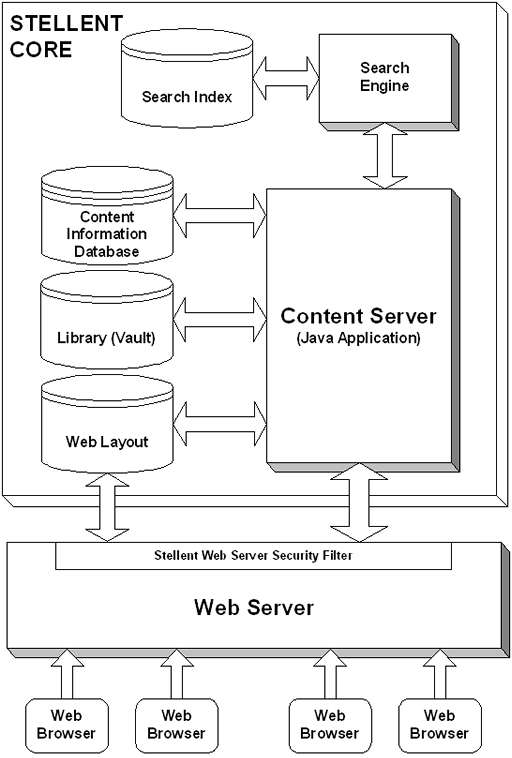
\includegraphics[width=0.5\textwidth]{bilder/basic_architecture.png}}
		\caption[Oracle UCM Architektur]{Oracle UCM Architektur\protect\footnote}
		\label{ucm-arch}
\end{figure}
\footnotetext{Quelle: \url{http://www.club-oracle.com/forums/oracle-universal-content-management-ucm-aka-stellent-t146/}}

Die Anwendung \gls{OracleUCM} ist aus folgenden Kernkomponenten aufgebaut:

\paragraph{Content Server}

Der Content Server ist das Herzstück der Oracle UCM Anwendung und basiert auf einer Java-Anwendung.
Er dient als Grundgerüst (Framework) für darüber liegende Funktionen, da er für die Ablage der Dokumente sowie der Verwaltung der drei Teilbereiche, siehe Abbildung \ref{lifecircle}, verantwortlich ist.

\begin{figure}[ht]
	\centering
	   \fbox{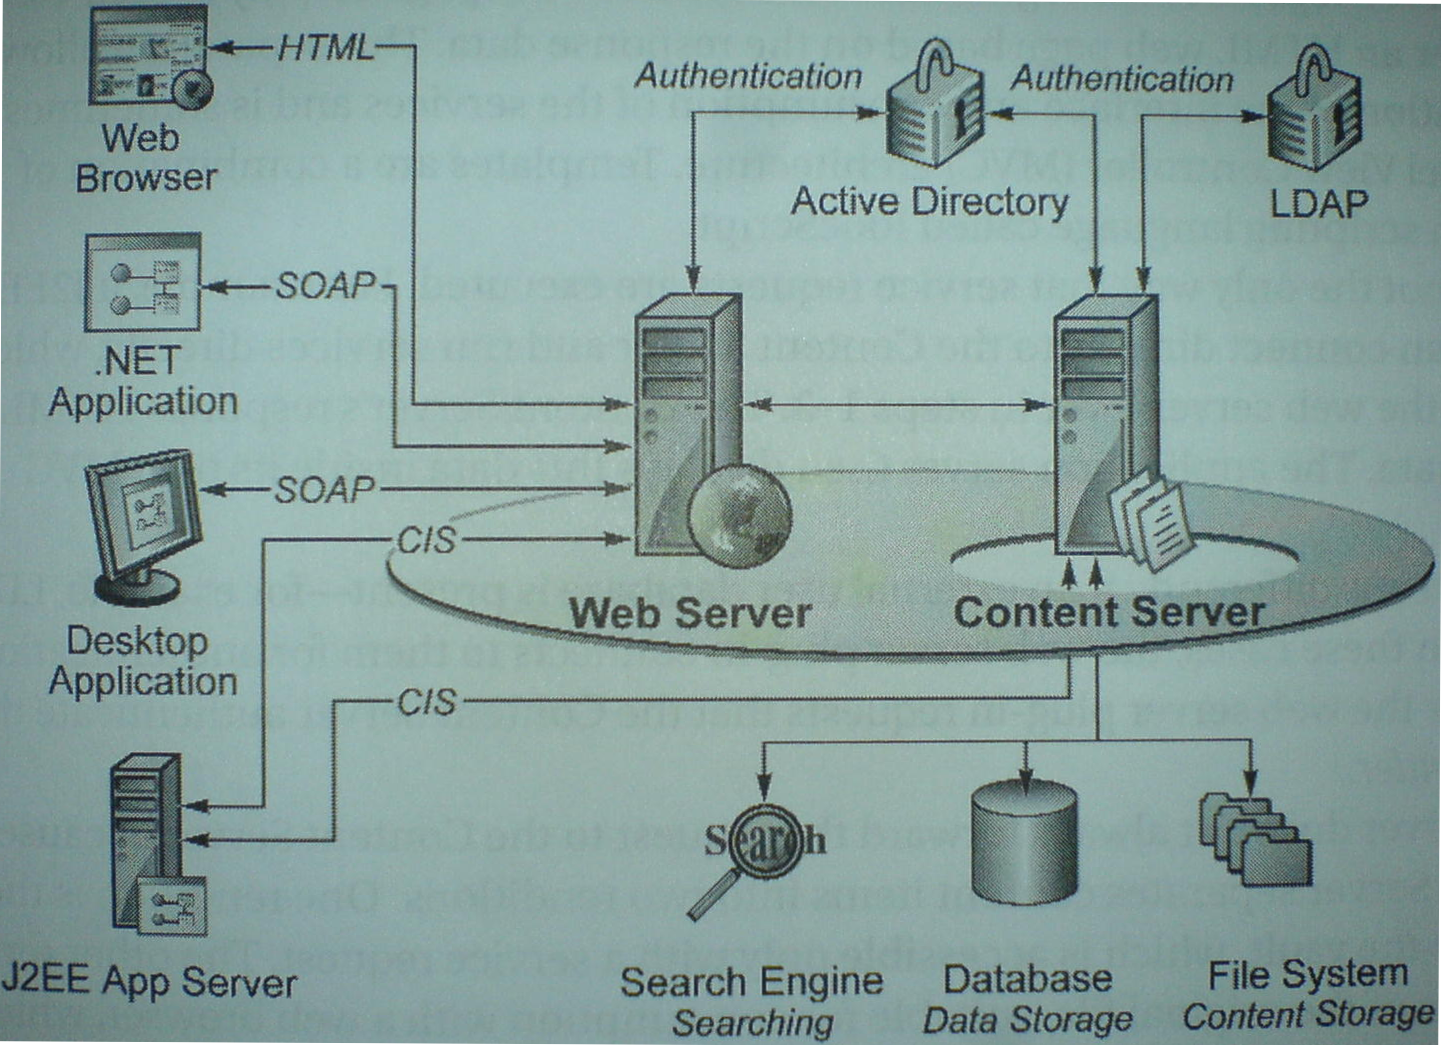
\includegraphics[width=0.85\textwidth]{bilder/contenserver.png}}
	  % \fbox{Quelle: \cite{Huff06} S. 17}
		\caption[Beispielhafter Einsatz eines Content Servers]{Beispielhafter Einsatz eines Content Servers\protect\footnote}
		\label{ucm-cs}
\end{figure}
\footnotetext{Quelle: \cite{Huff06} S. 17}

Dieses Framework ist als Service-Oriented Architecture (\gls{SOA}) aufgebaut.
Im Kontext des Content Servers wird als Service ein diskreter Aufruf einer Funktion verstanden.
Dabei kann diese Funktion das Hinzufügen, die Bearbeitung, die Konvertierung oder das Herunterladen eines Dokumentes bedeuten.
Diese Services und ihre einzelnen Funktionen werden durch das \gls{SOA}-Framework verdeckt und stehen als Web Service zur Verfügung.

Zusätzlich verwaltet der Content Server die Datenbank, die die Metadaten über die Dokumente beinhaltet.
Diese Metadaten werden für die Versionierung, Verwaltung und Suchanfragen verwendet.

\paragraph{Vault und Web Layout}
Der \textbf{Vault} ist ein Ordner auf dem Server in dem die Originaldateien der Benutzer in ihrem nativen Format gespeichert werden.
Im Gegensatz dazu werden im \textbf{Web Layout} die konvertierten Versionen der Dokumente abgelegt. Beispielsweise eine \gls{PDF}-Version einer Microsoft Word-Datei.

\paragraph{Search Engine}
Eine Suchanfrage eines Benutzers wird zuerst an den Webserver gesendet, der die Anfrage an den Content Server weitergibt.
Der Content Server verwendet anschließend seine Search Engine um ein Suchergebnis zu erhalten.
Das Suchergebnis wird wieder zum Webserver gesendet, der das Ergebnis an den Benutzer sendet.
Die Search Engine verwendet einen Suchindex, der aus den Metadaten und Referenzen zu den Volltextversionen der Dokumente besteht.

\paragraph{Webserver}
Der Webserver ist hauptsächlich für die Präsentation und Ausgabe der gespeicherten Dokumenten und Informationen zuständig.
Dabei ist er auch für die Authentifizierung der Benutzer zuständig.
\paragraph{Inbound Refinery}
Die Inbound Refinery ist für die Konvertierung der Dokumente zuständig und ist keine interne Komponente des Content Servers, sondern kann sich auch auf einem anderen Server befinden.
Dabei werden spezielle Add-ons (Filter) für die Konvertierung verwendet.
In zeitlichen Abständen überprüft die Inbound Refinery, ob die bisher eingecheckten Dokumente konvertiert werden müssen, und speichert die konvertierte Datei in den Web Layout-Ordner.

\subsection{Konkrete Verwendung / Einsatzgebiet}

\gls{OracleUCM} wird als \gls{ECM} für die Verwaltung von Webseiten, Dokumenten und Bilder im Forschungszentrum Karlsruhe eingesetzt.

Dabei wird im konkreten Anwendungsfall \gls{OracleUCM} als Bilddatenbank verwendet.
Diese Bilddatenbank nimmt Fotos und Bilder der Benutzer entgegen (\textit{Einchecken}) und konvertiert das Originalbild dabei in andere Bildversionen wie eine verkleinerte Version für Webseiten.

Dieser typische Ablauf soll durch Abblidung \ref{bdbanw} verdeutlicht werden.
\begin{figure}[ht]
	\centering
	   \fbox{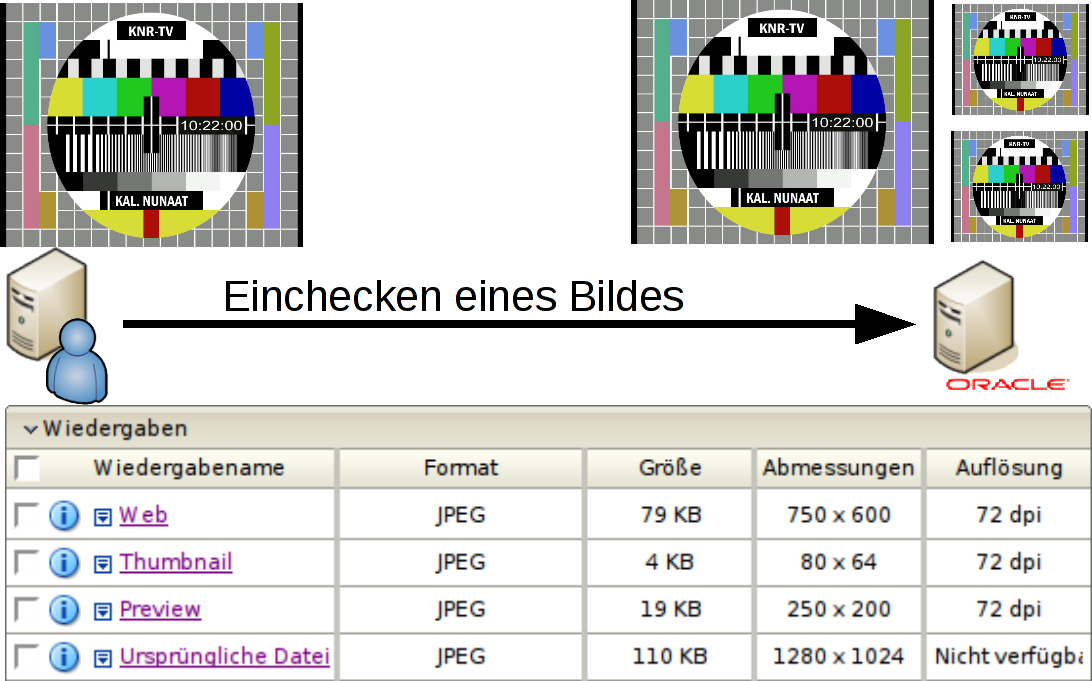
\includegraphics[width=0.85\textwidth]{bilder/bdb.png}}
		\caption{Bilddatenbank als Anwendung}
		\label{bdbanw}
\end{figure}

Die untere Tabelle zeigt die verschiedenen Bildversionen einer bereits konvertierten Bilddatei.\\

Da die Bilddatenbank unter einem Windows-Server betrieben werden soll, muss dies für die Überwachung bei der Auswahl der Überwachungselemente und Realisierung der Überwachung durch Nagios berücksichtigt werden.

\newpage
\section{Überwachungselemente}
Die Überwachung einer Dienstes über ein Netzwerk verteilt sich auf verschiedenen Ebenen mit unterschiedlichen Gewichtungen.
Zum Beispiel stellt das simple Senden eines Pings an den entsprechenden Server die niedrigste und primitivste Stufe dar, da hier lediglich die Netzwerkschnittstelle des Servers auf ihre Funktionalität und dabei der Status der Netzwerkstrecke getestet wird.(Rechner an und Netzwerk ok)
Ob die Anwendung überhaupt auf dem Server läuft und wenn, in welchem Zustand sie sich befindet (betriebsfähig, reagiert nicht mehr usw.), muss auf eine andere Weise herausgefunden werden.

Dabei lässt sich aus den verschiedenen Überwachungselemente folgende drei Kategorien bilden/ableiten:

\subsection{Statusabfragen}
\label{syschecks}
Diese Kategorie besteht aus einfacheren Überprüfungen, die jeweils den Status des Überwachungselementes überwachen.
Dabei können weitere Untergruppen gebildet werden:

\paragraph{System}
\begin{itemize}
\item \textbf{Ping} Überprüft, ob der Rechner vom Nagios-Server über das Netzwerk erreichbar ist.
\item \textbf{Prozessorauslastung} Überwacht die Auslastung des Prozessors und schlägt bei ungewöhnlich hohen Werten Alarm.
\item \textbf{Festplattenspeicherausnutzung} Überwacht die Speicherplatzauslastungen der verschiedenen Festplattenpartitionen, damit immer genügend Speicherplatz für Anwendungen und Betriebssystem verfügbar ist.
\item \textbf{Arbeitsspeicherauslastung} Beobachtet wie viel Arbeitsspeicher vom System verwendet wird und wieviel davon noch zur Verfügung steht.
\end{itemize}

\paragraph{Prozesse}
\begin{itemize}
\item \textbf{IdcServerNT.exe} Der Windowsprozess des Stellent-Servers
\item \textbf{IdcAdminNT.exe} Der Windowsprozess für die Administration (Webinterface?) des Stellent-Servers
\item \textbf{w3wp.exe} Der Windowsprozess des Microsoft "`Internet Information Services"'
\end{itemize}

\paragraph{Services}
\begin{itemize}
\item \textbf{IdcContentService???}  Den Zustand des "`Content-Dienstes"'-\pictext{sccdms01} überprüfen.
\item \textbf{IdcAdminService???}  Den Zustand des "`Administrations-Dienstes"'-\pictext{sccdms01\_admin} überprüfen.
\item \textbf{Zeitsynchronisationsdienst:} Überprüfen, ob der \pictext{W32TIME}-Dienst, der für den Zeitabgleich mit einem Zeitserver zuständig ist, läuft und die Abweichung zwischen Client und Zeitserver festhalten.
\item \textbf{Antivirusdienst}: Den Zustand den Dienstes überprüfen, der für die ständig Updates des Virusscanners Symantec AntiVirus notwendig ist.
\end{itemize}

\subsection{Überwachung der Funktionalität}
\label{funztest}
Durch die vorherigen Tests kann herausgefunden werden, ob eine Anwendung oder ein Dienst auf dem Server gestartet wurde.
Die Funktionalität kann durch solche Überprüfungen jedoch \textbf{nicht} sichergestellt werden.
Da beispielsweise der Prozess bzw. Dienst des Webservers gestartet ist, jedoch keine Webseite aufgerufen werden kann.
%Da beispielsweise der Webserver aufgrund eines kritischen Fehlers nicht erreichbar ist, der Prozess bzw. Dienst dennoch läuft.
Daher muss eine weitere Art von Überprüfungen/Checks die Anwendungen auf ihre Funktionalität (hin) überprüfen.

\begin{itemize}
\item \textbf{Webserver} Aufruf einer Webseite auf dem Server. Wenn auf diese Anfrage eine gültige Antwort in Form einer Statuscode-Meldung erfolgt, kann der reale/wirkliche Zustand des Webservers festgestellt werden.

\item \textbf{Webinterface des Oracle UCM} Zusätzlich wird mit dieser Abfrage die Integration des Content-Management-Systems in den Webserver überwacht, da hier nicht nur der Webserver, sondern eine UCM spezifische Webseite abgefragt wird.

\item \textbf{Benutzeranmeldung am Oracle UCM} Hier wird getestet, ob sich ein Benutzer erfolgreich am System anmelden kann.
Dies wird mit Anmeldungsdaten eines lokalen Benutzers und eines Active Directory-Benutzers durchgeführt um gleichzeitig/zusätzlich die Verbindung zum ADS-Server zu testen.

\item \textbf{Oracle Datenbank} Wenn keine Verbindung zur Oracle Datenbank möglich ist, können keine neuen Informationen gespeichert werden. 

%\item \textbf{Status von Cronjobs} In periodischen Zeitabständen werden Programme aufgerufen, deren Aufruf und Endstatus/Endergebniss überwacht werden muss. 
%Damit nicht das vorherige Ergebnis zu einem False Negative führt, müssen hier zusätzliche Zeitinformationen/zeitliche Parameter beachtet/bedacht werden.

\item \textbf{Anzahl Datenbankverbindungen} Anzahl der Verbindungen zur Datenbank, da aus Performanzgründen eine Obergrenze mit einer maximalen Anzahl festgelegt ist.
\end{itemize}

\subsection{Auswerten von Logdateien}
\label{checklog}
%Die zwei bisherigen Kategorien beinhalten simple Zustandsüberprüfungen oder aktive Funktionaltests.
In dieser Kategorie werden zusätzlich verschiedene Logdateien auf spezielle Warnungs- und Fehlermeldungen anhand eindeutigen Stopwörtern untersucht.
Dies ist notwendig um reaktiv Fehlverhalten der Anwendung zu erkennen, das nicht mit den vorherigen Überwachungselementen entdeckt wurde.
Des weiteren können durch die Analyse der Logdateien etwaige Alarmmeldungen der bisherigen Tests bestätigt, begründet oder aufgehoben werden.
Somit bietet das Auswerten der Logdateien zusätzliche Sicherheit False Positive- oder False Negative-Meldungen auszuschließen.

Die Oracle UCM Anwendung erstellt drei verschiedene Arten von Logdateien:\footnote{Quelle: \cite{UCMlog09}}

\begin{itemize}
\item \textbf{Content Server Log} 
\item \textbf{Inbound Refinery Log}
\item \textbf{Archiver Log}
\end{itemize}

Um alle Logs ohne Probleme im Internetbrowser anzuzeigen, liegen alle Logdateien im HTML-Format vor.
Alle drei Arten von Logs bestehen jeweils aus 30 verschiedenen Dateien, die sich täglich abwechseln.
Dadurch wird für jeden Tag im Monat eine separate Datei verwendet, um bei vielen Warnungs- und Fehlermeldungen durch die chronologische Anordnung/Hierarchie den Überblick zu behalten.
Dabei werden die Logdateien zwangsweise nach 30 Tagen nacheinander überschrieben.

Diese Rotation der Logdateien muss bei der Durchsuchung nach Signal/Stopwörter beachtet werden, damit stets die aktuelle Logdatei überwacht wird und keine veralteten Informationen für False Positives-Meldungen durch Nagios sorgen.

%wieso nur plugin check\_log und nicht einfahc umfangreicheres Standalone Programmw ie syslog\_nd oder 8pussy

\subsection{Benutzersimulation}

\begin{itemize}

\item \textbf{Einchecken von Dokumenten} Damit die eigentliche Aufgabe des Dokumentenverwaltungssystem überwacht werden kann, werden verschiedene Datenformate testweise eingecheckt. 
Dabei wird die Antwort der Anwendung auf das Hinzufügen der Dateien analysiert.

\item \textbf{Konvertierung} Da das hinzugefügte Dokument nicht nur einfach auf dem Server gespeichert wird, sondern dabei auch in ein anderes Format umgewandelt wird, muss diese Konvertierung zusätzlich überwacht werden. 
Wird beispielsweise ein Bild eingecheckt, wird dieses mehrfach in verschiedenen Auflösung oder als anderes Bilddateiformat gespeichert. 
Ob diese Transformation erfolgreich ablief, kann anhand dieser neuen Dateien festgestellt werden.

\item \textbf{Indizierung} Bei dem Einchecken sollen auch gleichzeitig zusätzliche Informationen über das Dokument festgehalten werden. 
Diese Informationen können beispielsweise der Name des Autors, das Erstellungsdatum der Datei oder - bei Bildern - der verwendete Farbraum sein. 
Bei der Suche nach einem Dokument können diese Informationen als zusätzliche Suchkriterien verwendet werden.
Daher müss überprüft werden, ob diese Daten richtig ausgelesen werden, der Datenbank hinzugefügt und vom Anwender abgefragt werden können. Dabei werden auch zuvor festgelegte/ausgewählte Testdateien verwendet.

\item \textbf{Suchfunktion} Nach einer erfolgreichen Indizierung muss das eingecheckte Dokument per Suchanfrage gefunden werden.
Ob die Suche und Indizierung erfolgreich abgelaufen ist, wird zusätzlich überprüft. 
\end{itemize}

Alle Überwachungselemente lassen sich inklusive ihrer Abhängigkeiten in einer Pyramide darstellen.

\begin{figure}[ht]
	\centering
	   \fbox{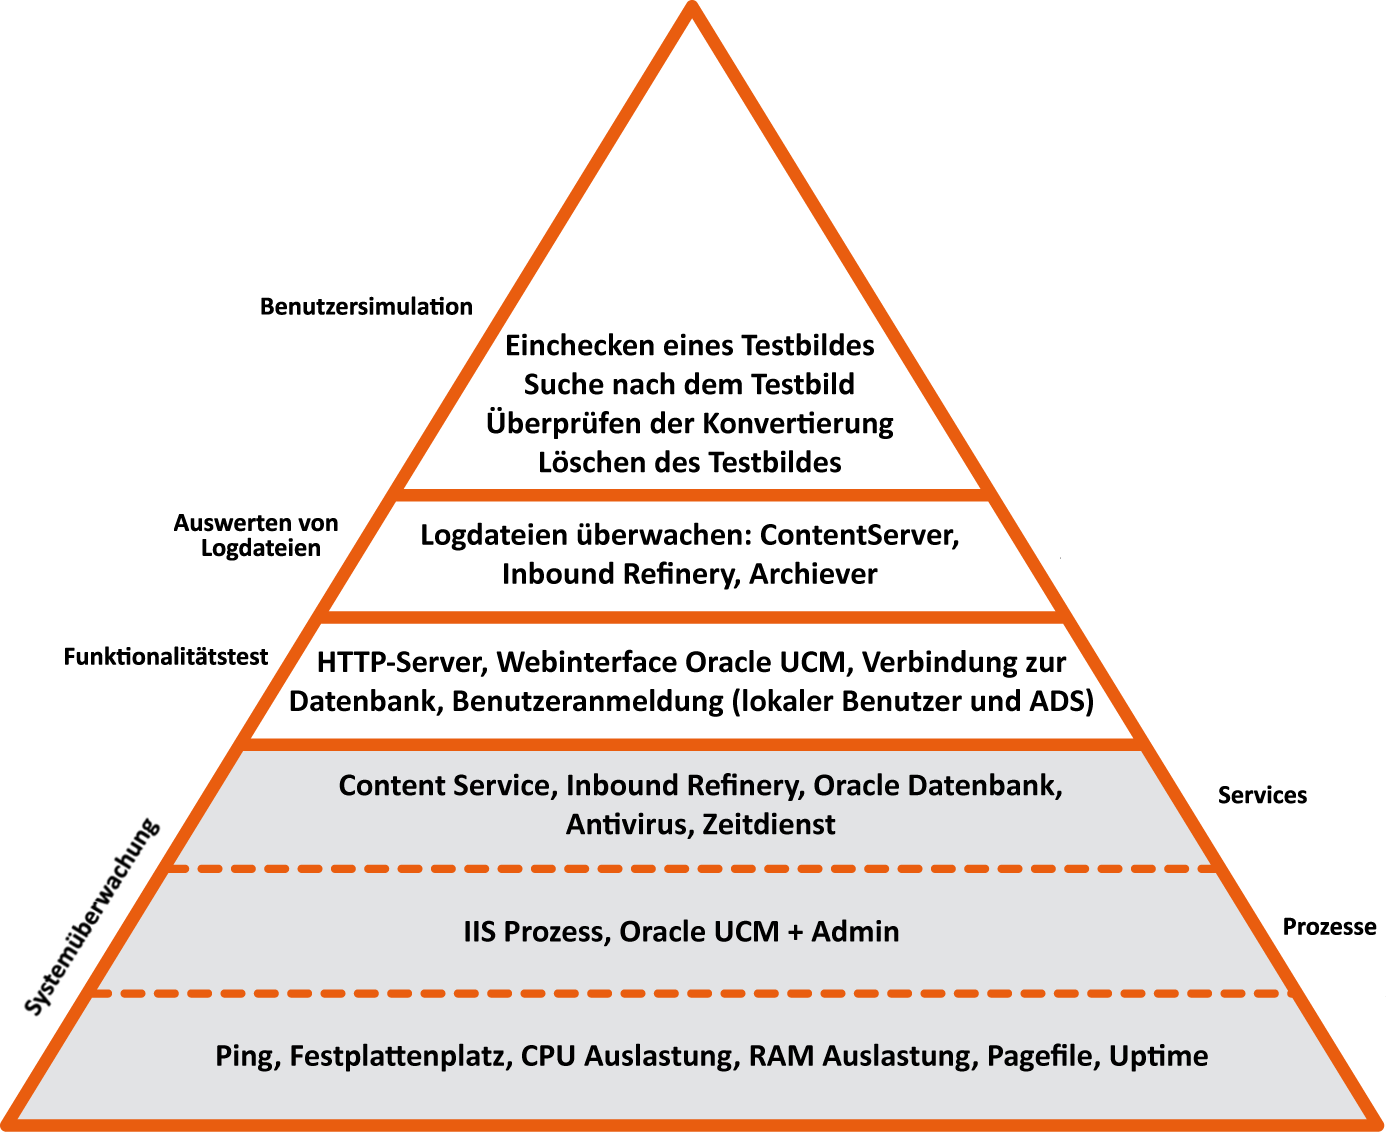
\includegraphics[width=1\textwidth]{bilder/pyramide_fertig2.png}}
		\caption{Überwachungselemente}
		\label{moniele}
\end{figure}


Die Basis für die alle anderen Tests bildet die Systemüberwachung.

An erster Stelle der Systemüberwachung steht die schlichte Erreichbarkeit über das Netzwerk per Ping.
Wenn der Server nicht erreichbar ist, können auch keine weiterführende Prüfungen durchgeführt werden.
Zur Systemüberwachung gehören auch allgemeine Informationen über die Systemressourcen wie freier Festplattenspeicher oder CPU Auslastung.

Die nächste Grundlage für die darüber liegenden Tests bildet die Überprüfung der laufenden Prozesse und der Status verschiedener Dienste bzw. Services.
Sollten bestimmte Prozesse nicht gefunden werden oder wichtige Dienste nicht gestartet sein, können auf diese Prozesse und Dienste aufbauende Checks nicht funktionieren.
Beispielweise kann der Funktionalitätstest der Benutzeranmeldung nicht realisierbar sein, wenn bereits zuvor in der Systemüberwachung der Prozess für den Webserver \gls{IIS} nicht gefunden werden konnte.













